\section{Descripci\'on del m\'odulo digital}

El siguiente diagrama de bloques muestra la configuraci\'on interna 
del aparato junto a sus caracter\'isticas t\'ecnicas.

\begin{figure}[!htb].
    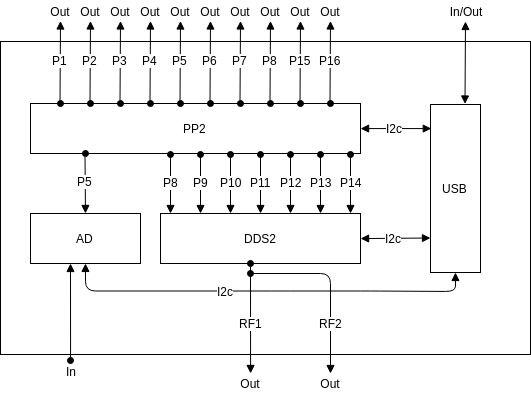
\includegraphics[width=\linewidth]{../figures/d6.jpg}
    \caption{Diagrama de bloques del m\'odulo digital}
    \label{fig:d6}
\end{figure}

\subsection{Salidas de pulsos TTL}
El usuario dispone de las salidas P1, P2, P3, P4, P6, P7, P15, P16. 
Las salidas P5, P8 si bien est\'an disponibles para su utilizaci\'on tienen 
una finalidad especial en el funcionamiento interno del m\'odulo que abordaremos m\'as 
adelante.

\subsection{Salidas RF}
Las salidas radiofrecuencia RF1 y RF2 son gemelas con un valor pico a pico de 200 milivoltios.

\subsection{Entradas AD}
Las entradas del conversor anal\'ogico digital son AD1 y AD2 correspondientes a los canales A y B respectivamente.
Admiten hasta 1.5 voltios de entrada.

\newpage
